%%% Local Variables:
%%% mode: latex
%%% TeX-master: t
%%% End:

\chapter{基于马来酰亚胺的光子晶体乙酰胆碱酯酶活性检测的研究}
\label{ch:maleimide}

\section{引言}
\label{sec:intro_maleimide}

乙酰胆碱酯酶(AChE)在人体中发挥重要的作用,它参与中枢神经信号传递,并通过对神经递质乙酰胆碱(ACh)水解而达到对神经信号的调控作用。
AChE的活性水平是人体活动的一个重要指标,例如AChE与不可逆抑制剂(例如有机磷农药、神经毒气)的结合会显著降低AChE的活性\cite{Ashani1992Mechanism,Tougu2001Acetylcholinesterase};而在阿尔滋海默症的治疗中,则又需要抑制AChE的活性以提高神经信号的表达程度\cite{Bartolini2003Amyloid}。针对AChE的高灵敏检测方法在生物、医药、化学等诸多方面均具有非常重要的应用价值\cite{Miao2010History}。
目前,已有一系列针对AChE活性的检测方法。
早期的Ellman试剂比色法\cite{Ellman1959Tissue,Ellman1961New}是一种简便的利用生物体活性硫化合物进行AChE活性的方法,但这种方法存在低灵敏度、时间长及假阳性信号等不足\cite{Rhee2003Qualitative}。近年来也有一些方法针对AChE的检测进行灵敏度的提高,包括单分子荧光标记物法\cite{Maeda200524Dinitrobenzenesulfonyl}、金胶体颗粒光学传感\cite{Pavlov2005Inhibition,Liu2012Highlya}、聚集诱导发光(AIE)\cite{Peng2009Fluorescence}、共轭高分子的比色或荧光法\cite{Feng2007Continuous,Li2011Fluorescence}以及电化学法\cite{Yissar2003Acetylcholine,Lu2011Novel}等。
这些方法提高了AChE的检测灵敏度,但由于大部分方法设计液相中的分子作用,不可避免地会受到实际样品中的电解质的电荷作用、荧光淬灭、以及金胶体颗粒团聚等问题干扰\cite{Levy2004Rational,Guo2013Oriented}。
同时上述液相的方法也存在操作困难、信号不直观等问题。

由于光子晶体自身的信号自表达特性、内部孔道结构以及聚合物材料的多样性,本章中我们将利用光子晶体来发展一种具有高灵敏度的AChE活性检测平台。
与Ellman方法的原理相近,我们采用ACh的模拟物乙酰巯基胆碱(ATCh)作为AChE的底物,通过化学反应将生成的含巯基的产物巯基胆碱(TCh)在光子晶体上形成信号表达。
因此,在这里我们所选用的目标反应为马来酰亚胺与巯基的Michael加成反应(\ref{fig:maleimide-thio-principle})。
\begin{figure}[b]
	\centering
	
\includegraphics[width=0.6\linewidth]{figures/ch3/michael_addition.png}
	\caption{马来酰亚胺-巯基反应原理示意图}
	\label{fig:maleimide-thio-principle}
\end{figure}
由于马来酰亚胺的共轭结构,容易与巯基发生加成反应,且这种加成反应可以在中性pH条件下常温发生,适于实时的检测需求\cite{Marrian1949322};同时,在中性条件下,马来酰亚胺与巯基的反应存在特异性,不会与氨基发生Michael加成反应(氨基与马来酰亚胺反应需在较高pH(>10)条件下进行),适于AChE水解产物的特异性检测。
结合上述考虑,本章中将利用含马来酰亚胺的聚合物制备反蛋白石光子晶体材料,并用于AChE的活性检测。

本章中利用光子晶体进行AChE的活性的检测的基本原理如图~\ref{fig:maleimide-photonic-principle}。
首先,利用模板复制法制备具有马来酰亚胺(含保护基)基团的反蛋白石材料,并通过脱保护反应获得具有化学活性的马来酰亚胺功能聚合物反蛋白石薄膜。这种活性光子晶体材料能够与AChE的水解产物TCh发生Michael加成反应。
由于TCh的胆碱头基具有正电荷,因此反应后的聚合物光子晶体内部的Donan电势增高,从而造成聚合物的吸水膨胀。
这种由于化学反应造成的聚合物亲疏水变化带来了光子晶体晶格常数的变化,最终导致了光子晶体禁带的偏移,即将酶的活性信息转化为能够肉眼观察的光学信号而表达出来。
本章的其他部分将对这种光子晶体材料的制备、表征及性能等方面进行更为详尽的介绍。
\begin{figure}[htbp]
  \centering
  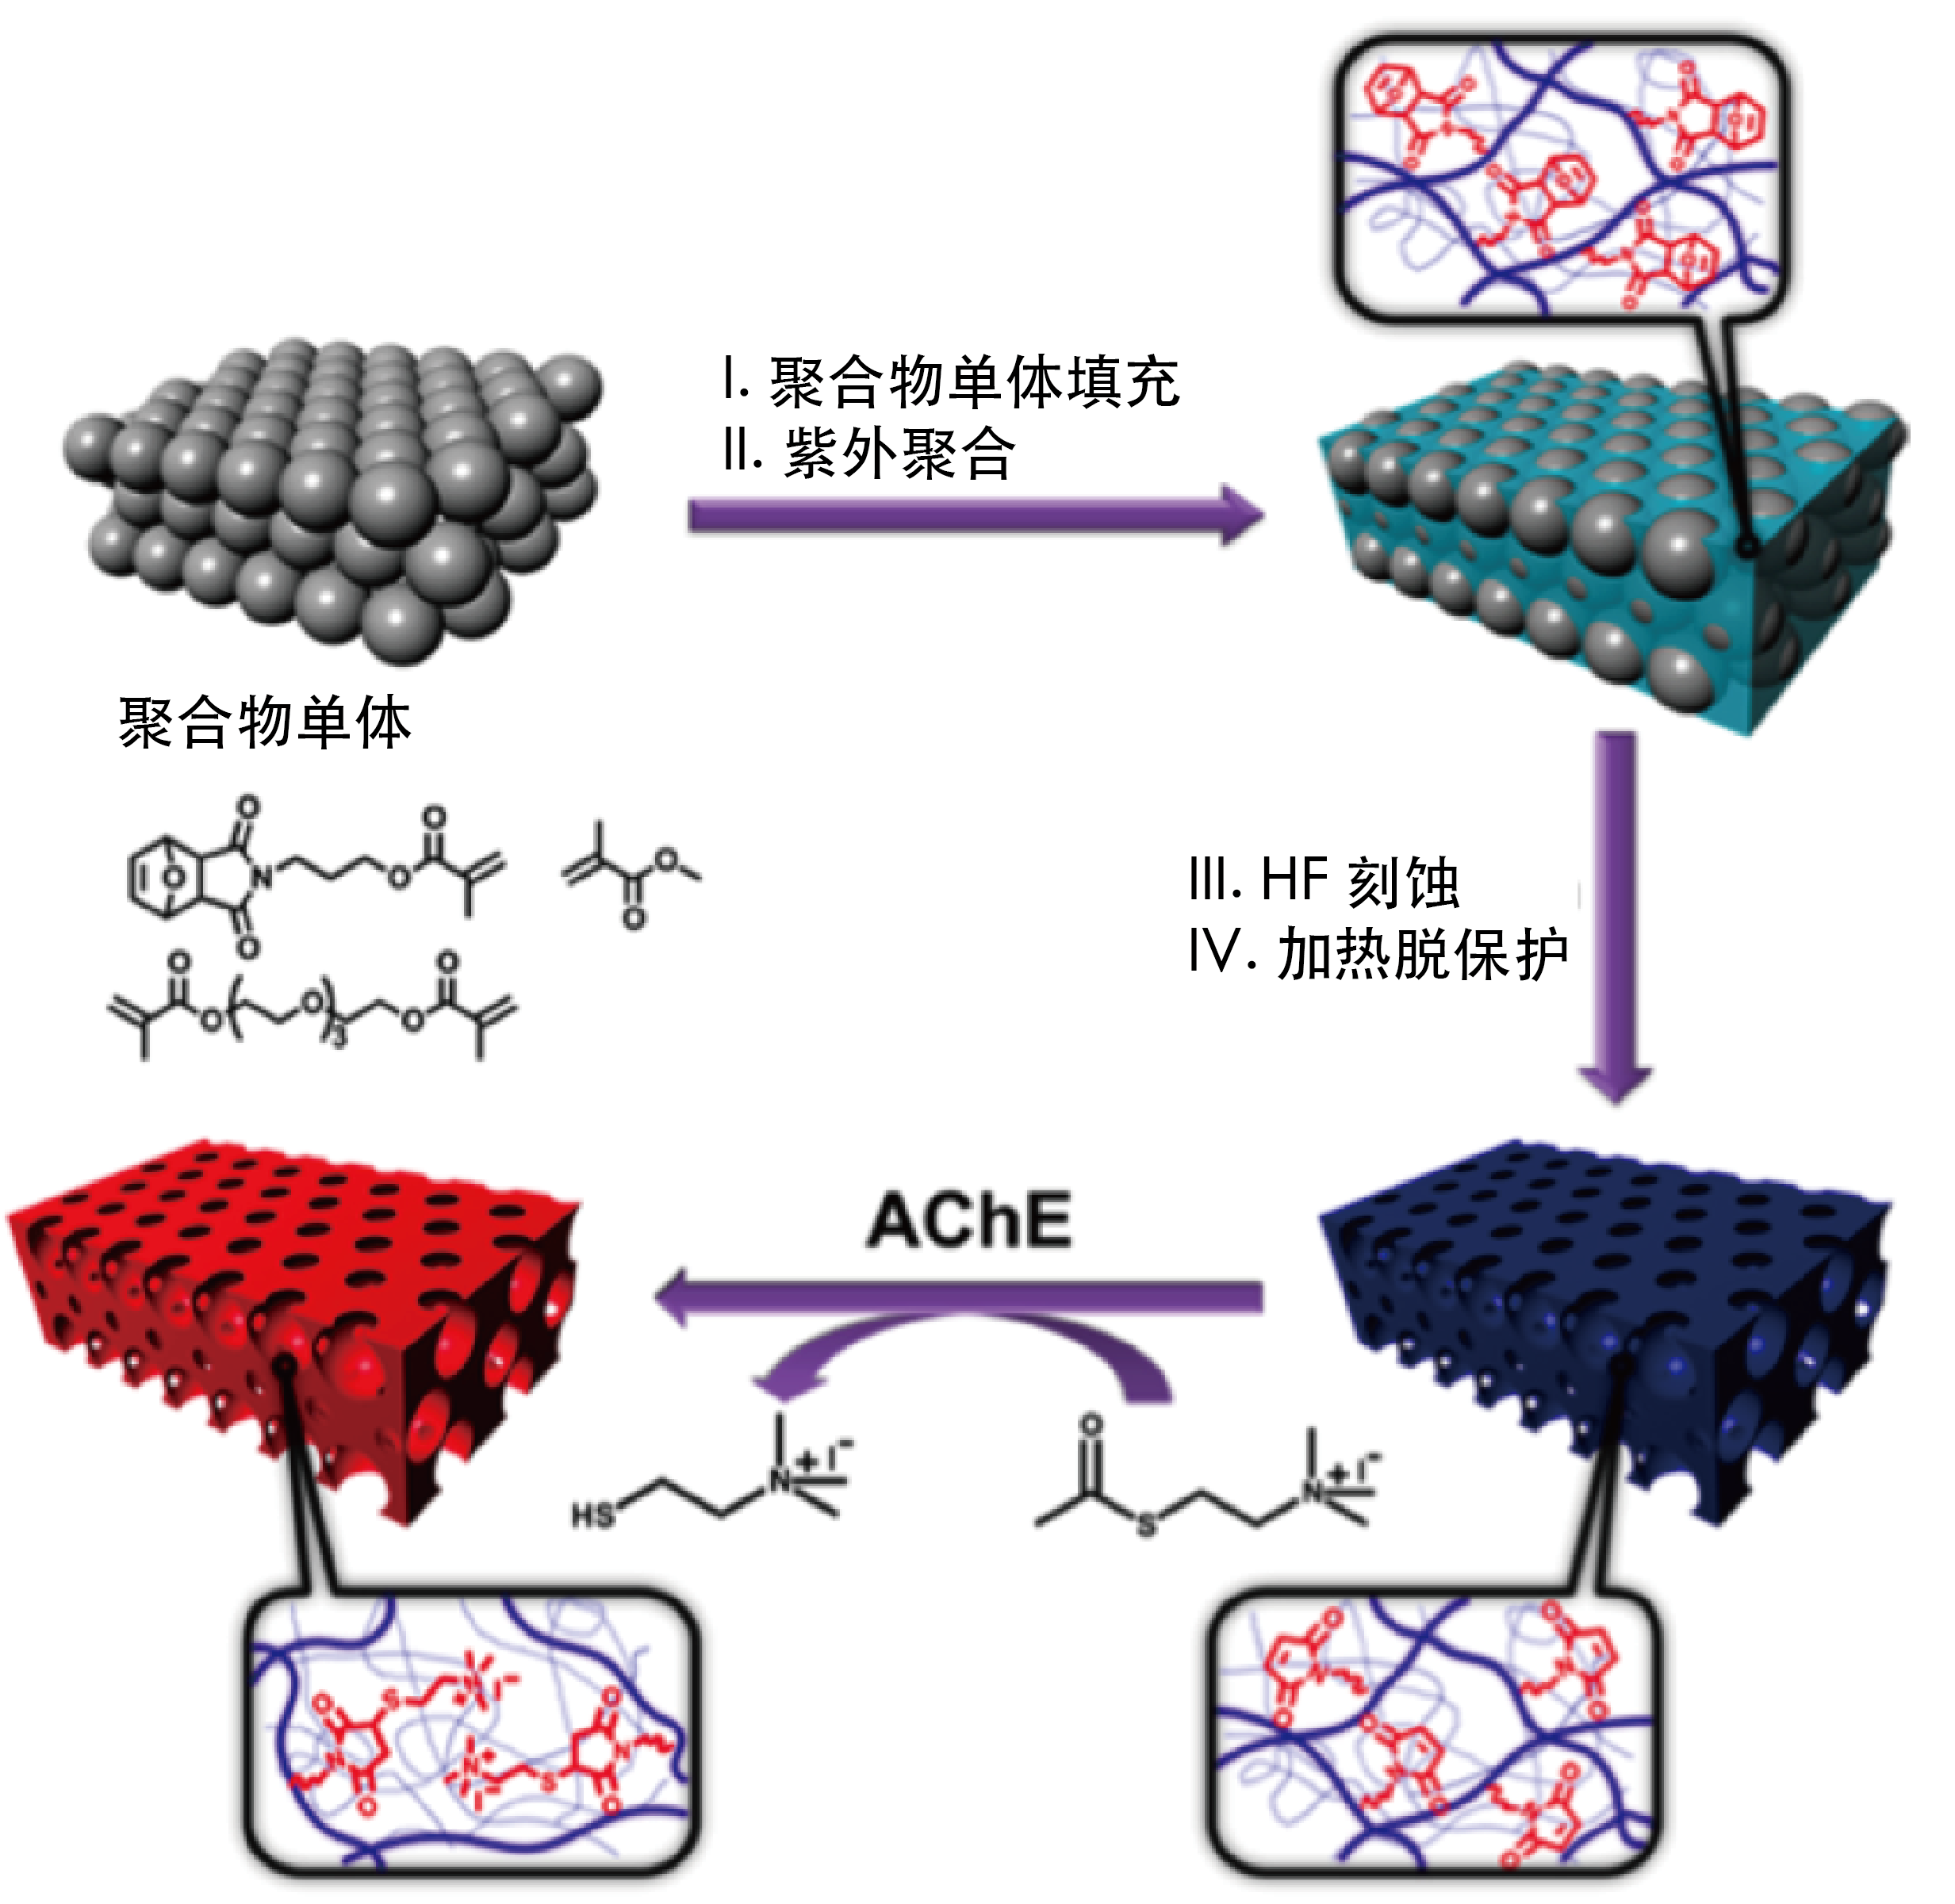
\includegraphics[width=0.85\linewidth]{figures/ch3/principle.png}
  \caption{含马来酰亚胺光子晶体平台对AChE活性检测的原理示意图}
  \label{fig:maleimide-photonic-principle}
\end{figure}

\section{实验部分}
\label{sec:ch3-exp}

\subsection{实验材料与仪器}
本章中所使用的实验材料与仪器分别见表~\ref{tab:ch3-material}与表~\ref{tab:ch3-instrument}。常用的制备仪器如玻璃器皿、搅拌器等这里不再赘述,下同。

\begin{table}[htbp]
  \centering
  \caption{本章所用实验材料}
  \label{tab:ch3-material}
    \begin{tabularx}{\linewidth}{XXXX}
      \toprule[1.5pt]
      {\heiti 药品名称} & {\heiti 纯度} & {\heiti 来源} & {\heiti 处理方法}\\
      \midrule[1pt]
      二氯甲烷 & 分析纯 & 国药集团化学试剂有限公司 & 用前重蒸\\
      三乙胺(TEA) & 分析纯 & 国药集团化学试剂有限公司 & 直接使用\\
      Exo-3,6-环氧-1,2,3,6-四氢邻苯二甲酸酐& 98\% & Alfa Aesar & 直接使用\\
      3-氨基-1-丙醇 & 98\% & Alfa Aesar & 直接使用\\
      甲基丙烯酸甲酯(MMA) & 98\% & Alfa Aesar & 直接使用\\
      四乙二醇二甲基丙烯酸酯(TEGDMA) & 98\% & Alfa Aesar & 直接使用\\
      2-羟基-2-甲基-1-苯丙酮(HMPP) & 98\% & Acros Organics & 直接使用\\
      氢氟酸 & w/w\%=40\% & Acros & 直接使用\\
      去离子水 & 分析纯 & 自制 & 直接使用\\
      乙酰胆碱酯酶(AChE)& >700 U/mg & Sigma-Aldrich & 直接使用\\
      丁酰胆碱酯酶(BChE)& >200 U/mg & Sigma-Aldrich & 直接使用\\
      溶菌酶(Lyz)& >1000 U/mg & Sigma-Aldrich & 直接使用\\
      碘代乙酰巯基胆碱 & 98\% & Sigma-Aldrich & 直接使用\\
      碘代丙锭 & 98\% & Sigma-Aldrich & 直接使用\\
      塔克林 & 98\% & Sigma-Aldrich & 直接使用\\
      多萘哌齐 & 98\% & Sigma-Aldrich & 直接使用\\
      \bottomrule[1.5pt]
    \end{tabularx}
\end{table}

\begin{table}[htbp]
  \centering
  \caption{本章所用仪器}
  \label{tab:ch3-instrument}
    \begin{tabularx}{\linewidth}{XXX}
      \toprule[1.5pt]
      {\heiti 仪器名称} & {\heiti 仪器型号} & {\heiti 厂家} \\
      \midrule[1pt]
      反射光纤光谱仪 & USB2000 & OceanOptics\\
      场发射扫描电子显微镜(SEM) & LEO-1503 & Bruker\\
      傅里叶变换红外光谱仪(FTIR)& PE 2000 & Perkin-Elmer\\
      核磁共振仪(NMR) & ECA 300 &JEOL\\
      电喷雾质谱仪(ESI) &Esquire-LC &Bruker\\
      接触角测定仪 & OCA 20 &Dataphysics\\
      \bottomrule[1.5pt]
    \end{tabularx}
\end{table}


\subsection{含马来酰亚胺的丙烯酸酯功能单体合成}

由于马来酰亚胺基团的双键活性较高,在自由基聚合中不稳定,因此需要对其进行保护。这里采用呋喃官能团进行保护,而同时这种保护基也可以由逆Diels-Alder反应来去除。
基于上述考虑,我们设计了含保护的马来酰亚胺的丙烯酸酯功能单体。其合成步骤如图~\ref{fig:maleimide-sync}:
\begin{figure}[htbp]
  \centering
  
\includegraphics[width=\linewidth]{figures/ch3/ch3-maleimide-synth.png}
  \caption{含马来酰亚胺的丙烯酸酯功能单体的合成步骤}
  \label{fig:maleimide-sync}
\end{figure}

对应的化合物合成方法如下:

化合物1:将3.32 g (20 mmol, 1 eqiv)Exo-3,6-环氧-1,2,3,6-四氢邻苯二甲酸酐与7.50 g (100 mmol,5 eqiv)3-氨基-1-丙醇混合于100 mL的圆底烧瓶中,并在80 \text{$^\circ$}C油浴条件下剧烈搅拌4 h。反应停止后,将粘稠的粗产物溶解于100 mL CH\text{$_2$}Cl\text{$_2$}中,并分别用1 M稀盐酸、饱和NaCl溶液洗涤一次。
分离的有机相用MgSO\text{$_4$}干燥。将有机相旋蒸真空干燥,得到一白色固体(1.59 g,35.7\%)。
化合物1:2-(3-羟丙基)-3a,4,7,7a-四氢-4,7-环氧异吲哚-1,3-二酮,\text{$^1$}H-NMR(300 MHz,CDCl\text{$_3$}): \text{$\delta$} 6.53 (s, 2H, -CH=), 5.28 (s, 2H, −CH−O−), 3.65 (t, −N−CH\text{$_2$}−, 2H), 3.53 (t, −CH2−O−, 2H), 2.88 (m, 2H, −CHCO−), 2.50 (s, 1H, −OH), 1.77 (m, 2H, −CH\text{$_2$}CH\text{$_2$}CH\text{$_2$}−)。ESI-MS: 246.1 [M+Na]\text{$^+$}。

化合物2:将0.90 g(4.04 mmol,1eqiv)化合物1与2 mL三乙胺(TEA)溶解于20 mLCH\text{$_2$}Cl\text{$_2$}中,在冰浴搅拌条件下,向溶液中缓慢滴加甲基丙烯酰氯。
滴加完毕后向反应体系中通入氮气,使其在室温下继续搅拌过夜。
反应完成后,将反应液用CH\text{$_2$}Cl\text{$_2$}稀释至约100 mL,并分别用水、饱和NaCl溶液洗涤一遍。用MgSO\text{$_4$}干燥后,将有机相浓缩并以2:1 的石油醚(PE):乙酸乙酯(EA)展开液进行柱层析分析。
旋蒸干燥后得到灰白色蜡状固体(1.03g,87.5\%)。化合物2:3-(1,3-二氧代)-3a,4,7,7a-四氢-4,7-环氧异吲哚基丙基甲基丙烯酸酯,\text{$^1$}H-NMR(300 MHz,CDCl\text{$_3$}):\text{$\delta$} .51 (s, 2H, −CH=CH−), 6.13 (s, 1H, =CH\text{$_2$}), 5.57 (s, 1H, =CH\text{$_2$}), 5.26 (s, 2H, −CHO−), 4.12 (t, 3H, −CONCH\text{$_2$}−), 3.61 (t, 3H, −COOCH\text{$_2$}−), 2.84 (m, 2H, −CHCO−), 1.97 (m, 5H, −CH\text{$_3$}−CH\text{$_2$}−)。ESI-MS: 292.1 [M+H]\text{$^+$}。


\subsection{含马来酰亚胺反蛋白石光子晶体功能材料的制备}
反蛋白石光子晶体的制备方法与\ref{subsec:evap-template}节中的方法类似。
其基本原理叙述如下:

1. 将马来酰亚胺功能单体(分子2)0.289 g (1 mmol)、0.100 g (1 mmol)MMA、及0.152 g (0.5 mmol)四乙二醇二甲基丙烯酸酯(TEGDMA)混合溶解均匀,并加入1 \%摩尔分数的2-羟基-2-甲基-1-苯丙酮(HMPP)光引发剂作为聚合物预聚液,并进行脱气处理,除去其中残留氧气。

2. 将SiO\text{$_2$}光子晶体模板(利用溶剂挥发垂直沉积法制备)与相同大小的两片载玻片制作三明治复合结构,并用毛细作用将预聚液吸收入光子晶体缝隙中,直至光子晶体变为透明为止。

3. 将复合结构置于UV灯下聚合5 min,待其冷却后,将光子晶体复合模板放入5 \%HF溶液中进行刻蚀约30 min,直至具有光子晶体结构色的游离有机物薄膜从玻璃片中脱离。

4. 将上述得到的反蛋白石光子晶体游离薄膜用乙醇-去离子水清晰干燥。最后将反蛋白石薄膜放入含甲苯的圆底烧瓶中并在120 $^{\circ}$C条件下回流12 h,以去除马来酰亚胺基团的保护基。经过脱保护处理的光子晶体薄膜便能够用于进行AChE酶活性的检测。

\subsection{含马来酰亚胺光子晶体对AChE的响应检测}
将上述制备的马来酰亚胺反蛋白石光子晶体薄膜切割为约 3 \text{$\times$} 3 cm\text{$^2$}大小,并转移到黑色的双面防水胶带上,并粘贴到高约0.5 cm的96孔板格道底以制备AChE检测的基本单元。根据实验的不同测定需求,将含AChE、ATCh或AChE抑制剂的缓冲液配制至1 ml,并加入对应的孔中。在经过一定时间的摇床震荡之后,用反射式光纤光谱仪测定光子晶体的反射光谱。对于不同的实验需求,所使用的AChE缓冲液的配置分别如下:

1. 对于AChE活性的检测应用,维持ATCh的浓度为1 mM,AChE的浓度从10 mU/mL至10 U/mL。反射光谱的测定在AChE反应30 min之后测定。

2. 对于酶选择性检测,ATCh的浓度维持为1 mM,AChE、BChE与Lyz的浓度维持 1 U/mL。反射光谱的测定同样在反应30 min后测定。

3. 对TCh标准工作曲线的测定,ATCh的浓度从10\text{$^{-9}$}-10\text{$^{-3}$} M不等,AChE的浓度维持在 1 U/mL 以确保ATCh完全分解。光子晶体的光谱在光子禁带的偏移稳定后进行测定(30-60 min)。

4. 对AChE的酶动力学参数测定,AChE浓度为 1 U/mL,ATCh浓度分别为5\text{$\times$}10\text{$^{-6}$}、1\text{$\times$}10\text{$^{-6}$}、5\text{$\times$}10\text{$^{-7}$}、1\text{$\times$}10\text{$^{-7}$} mol/L。分别测定光子晶体禁带在上述浓度下随时间的变化关系,并利用标准工作曲线转化为ATCh的分解速率,并通过起始数据点计算酶反应的初始速率。

5. 对AChE抑制剂的检测,将1 U/mL浓度的AChE缓冲液分别与不同浓度(10\text{$^{-9}$}-10\text{$^{-4}$} mol/L)的AChE抑制剂(碘化丙锭、多萘哌齐、塔克林)混合,在常温摇床上混合30 min以促进抑制剂与酶的结合,并将底物ATCh(1 mmmol/L)与上述溶液混合,测定含马来酰亚胺光子晶体薄膜在上述溶液中的光子禁带偏移,并根据不同的抑制剂浓度绘制抑制剂的抑制曲线,计算抑制剂抑制能力。

\section{结果与讨论}
\subsection{含马来酰亚胺聚合物反蛋白石光子晶体的表征}

我们首先对含马来酰亚胺的光子晶体材料进行表征。如
	图~\ref{fig:maleimide-character}A-图~\ref{fig:maleimide-character}C
所示,经过了光子晶体模板复制、去除以及加热脱保护等步骤之后,光子晶体的fcc排列结构能够很好的保持,说明制备过程中的加热等操作对聚合物膜结构影响较小。且在薄膜的总体结构上保持了完整的孔道结构。
制备后的反蛋白石光子晶体的Bragg衍射峰较SiO\text{$_2$}模板有一定的蓝移(605 nm -> 512 nm),且具有相似的品质因子(Q=8.82),说明了制备的反蛋白石光子晶体具有良好的光学性质,能够作为信号自表达的传感材料(图~\ref{fig:maleimide-character}D)。
\begin{figure}[htbp]
  \centering
  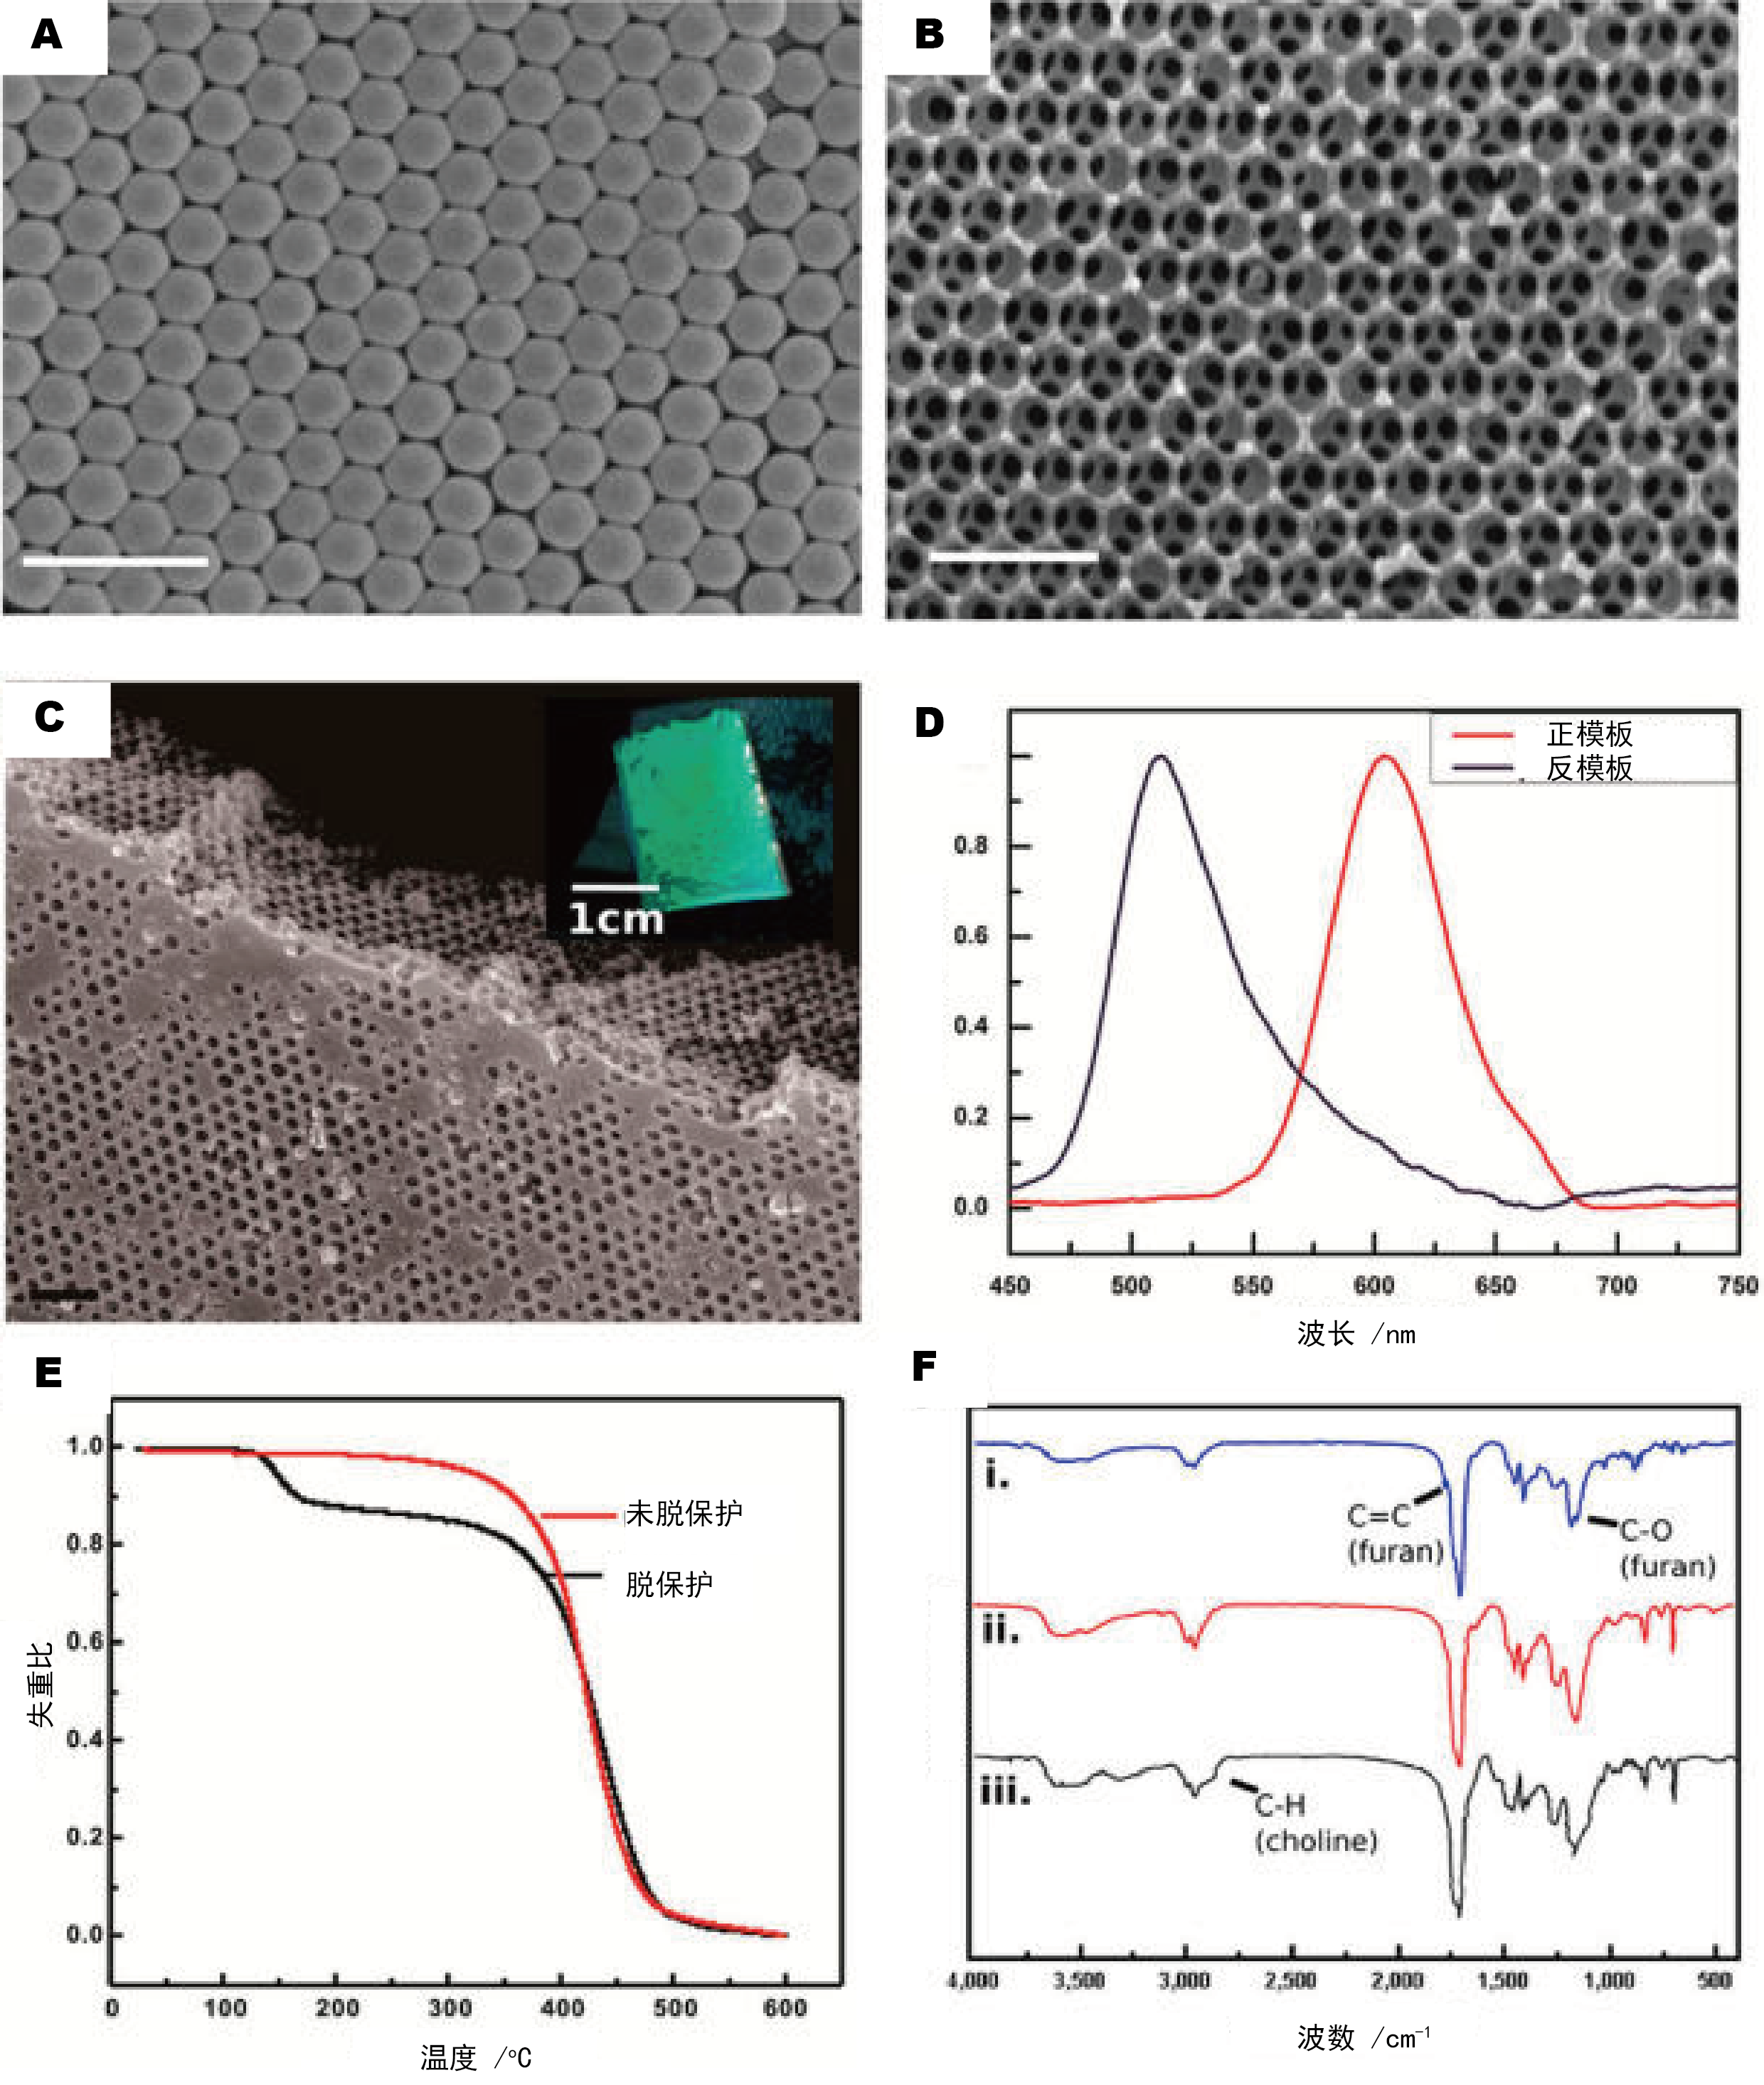
\includegraphics[width=\linewidth]{figures/ch3/material-maleimide.png}
  \caption{含马来酰亚胺的聚合物光子晶体的表征。(a). SiO\text{$_2$}光子晶体模板的SEM照片;(b) 反蛋白石光子晶体的正面SEM照片;(c) 反蛋白石光子晶体侧面照片及实物图片;(d) SiO\text{$_2$}模板与反蛋白石光子晶体的Bragg衍射峰;(e) 含马来酰亚胺聚合物脱保护前后的TGA曲线; (f) 含马来酰亚胺聚合物脱保护及反应前后的红外谱图。}
  \label{fig:maleimide-character}
\end{figure}

由于马来酰亚胺中的双键在自由基聚合过程中不可避免地会参与反应,因此这里采用了呋喃保护的马来酰亚胺聚合单体。在聚合完成之后采用加热逆Diels-Alder反应来脱去呋喃保护基团。
这里我们采用多重表征方法来表征呋喃保护基团的离去程度。首先,我们利用热重分析(TGA)来表征(图~\ref{fig:maleimide-character}E)。未经过加热脱保护处理的聚合物在加热条件下在100-200 $^{\circ}$C范围内有11.9 \%的重量损失,对应了呋喃官能团的离去,且其含量与聚合物中的呋喃官能团含量(12.4 \%,按预聚液组分计算)相近;
同时,经过热处理后的聚合物则直到400 $^{\circ}$C才开始显示出热分解。结合上述两点说明经过热处理的脱保护是充分的。
此外,红外光谱(IR)也能够表明保护基的脱去(图~\ref{fig:maleimide-character}F)。在未脱去保护基的聚合物中,1783 cm\text{$^{-1}$}的肩峰代表了呋喃官能团的C=C弯曲震动,而在1158 cm\text{$^{-1}$}的峰则代表了呋喃中C-O的伸缩振动。而在经过热处理的聚合物红外谱中可以观察到两个对应峰均消失,证明了呋喃基团的充分离去。

此外,我们也对这种含马来酰亚胺的反蛋白石光子晶体对AChE的响应性。首先我们用1 mM ATCh与10 U/mL AChE的PBS缓冲溶液对光子晶体进行处理,并测定了其红外光谱与接触角。
由于马来酰亚胺的弱C=C振动吸收与羰基的强吸收峰存在重叠,不能直接利用C=C振动吸收峰的变化来表征马来酰亚胺的反应\cite{Aguiar2011Theoretical}。
这里我们采用观察Michael加成后的胆碱基团特征峰来表征反应的进行。注意到在2869 cm\text{$^{-1}$} 处出现了新的肩峰,对应了胆碱基团上存在的多个甲基及亚甲基基团(图~\ref{fig:maleimide-character}F)。
同时,接触角测试进一步表征了聚合物在AChE水解反应后的组成变化。如图~\ref{fig:maleimide-CA}所示,聚合物的接触角由反应前的85.9$^{\circ}$降低至反应后的8$^{\circ}$,这种急剧的亲疏水性变化是由胆碱基团的Michael加成造成的。
同时,可以注意到在接触角的测试过程中,液面的变化是一个缓慢的过程,从疏水性的的大接触角阶段过渡到低接触角的阶段时间为若干分钟,而同样的液面平衡在普通平面材料上则很短。
这种变化是由于反蛋白石光子晶体内部的孔道结构造成的,间接证明了光子晶体内部的孔道结构。
\begin{figure}[htbp]
  \centering
  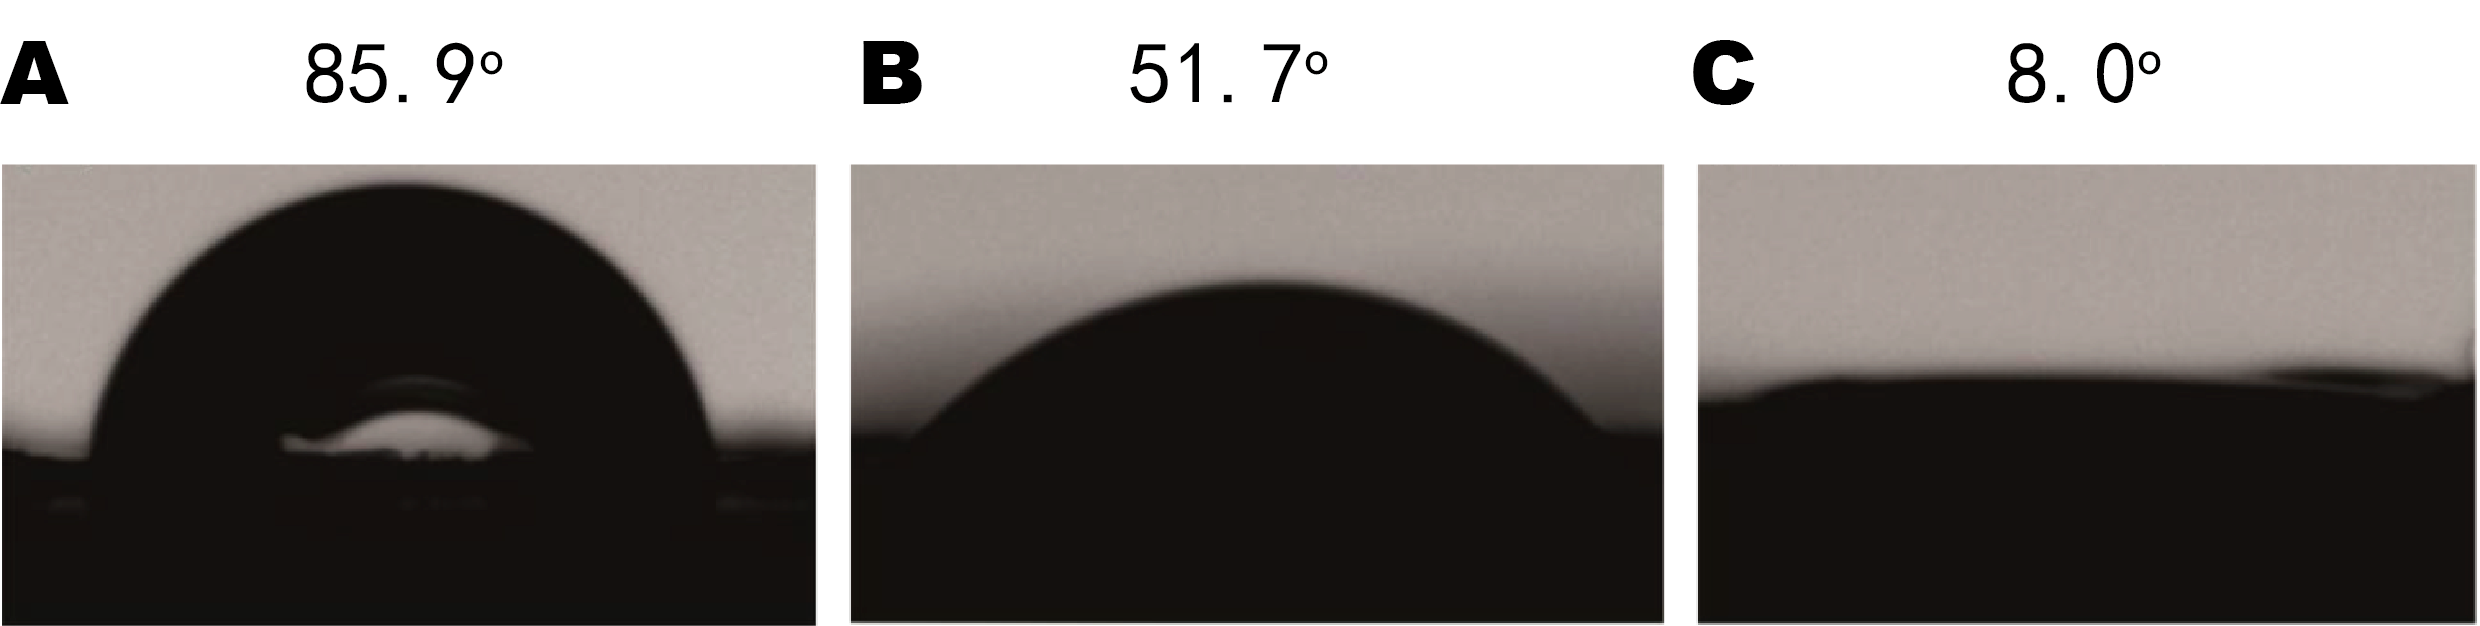
\includegraphics[width=\linewidth]{figures/ch3/maleimide-CA.png}
  \caption{含马来酰亚胺的光子晶体与TCh反应前后的接触角变化。A. 未反应的光子晶体;B. 反应后光子晶体液面平衡中;C. 液面平衡后的光子晶体。}
  \label{fig:maleimide-CA}
\end{figure}

\subsection{光子晶体平台对AChE的检测性能}
我们进一步研究了这种光子晶体检测平台的检测性能。由于酶反应是时间相关的过程,我们首先研究了在不同底物条件下的光子禁带变化过程以确定光子晶体的稳态平衡时间。
\begin{figure}[htbp]
  \centering
  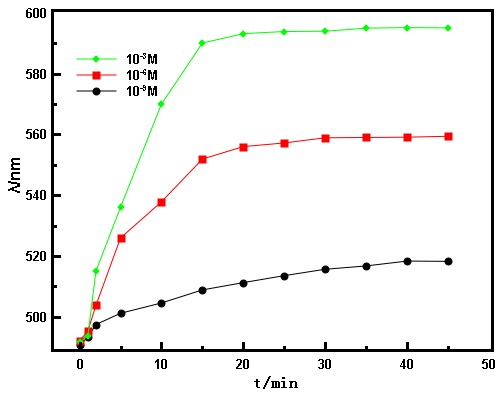
\includegraphics[width=0.6\linewidth]{figures/ch3/saturation_curve.png}
  \caption{光子晶体对不同底物浓度情况下的响应速率}
  \label{fig:maleimide-saturation}
\end{figure}

如图~\ref{fig:maleimide-saturation},在30 min之中,光子晶体Bragg衍射峰在较高的底物浓度下(10$^{-3}$、10$^{-6}$ mol/L)能够达到稳态;而在更低的底物浓度(10$^{-9}$ mol/L)情况下,Bragg衍射峰的偏移能够达到约90 \%。
因此在这里确定了基础的反应时间为30 min,而在较低的反应浓度之下则对Bragg衍射峰进行实时测量直到达到最大值为止。
由于这里重要的参数是光子晶体Bragg衍射峰的位置或偏移量,对其强度并不用特殊处理,因此所测量的反射光谱均进行归一化处理以便于分析。

基于上述实验参数我们研究了光子晶体对AChE的响应性。
如图~\ref{fig:maleimide-enzyme}A所示,未反应的光子晶体薄膜的Bragg衍射峰为505.7 nm,呈现出蓝色的结构色;经过2.5 U/mL AChE 及1 mM ATCh处理后,Bragg衍射峰红移至569.3 nm而呈现出绿色的结构色;当AChE浓度提高至10 U/mL时,Bragg衍射峰进一步红移至634.4 nm而呈现出红色的结构色。
从上述实验现象中可以看出,含马来酰亚胺的光子晶体材料能够对不同活性水平的AChE产生响应,并且反映为可用肉眼直接观察的结构色信号。
进一步地,我们将AChE的浓度从10 mU/mL 到 10 U/mL变化,来研究这种光子晶体平台的检测性能(图~\ref{fig:maleimide-enzyme}B)。
对不同浓度下的光子晶体Bragg衍射峰位移进行曲线绘制,可以发现其Bragg衍射峰位移随着AChE浓度增加而减慢(图~\ref{fig:maleimide-enzyme}C),而在低浓度区域下呈现近似线性的特性。
同时,我们将测定曲线外延至零点,以计算该体系的检测极限(LOD)。
以实验所使用的光纤光谱仪系统误差(2 nm)作为参考值,在3倍噪声水平(6 nm)上对应的AChE活性为5 mU/mL,即为该光子晶体平台检测极限(LOD)。
值得注意的是,这种方法的LOD值在现有的报道方法中处于较高的水平,高于比色法\cite{Li2011Colorimetric}的水平,同时能够媲美荧光标记法\cite{Pavlov2005Inhibition,Feng2007Continuous}或AIE法\cite{Peng2009Fluorescence},证明了这种结合化学反应与光子晶体光学性质的检测平台的高灵敏性。
\begin{figure}[htbp]
  \centering
  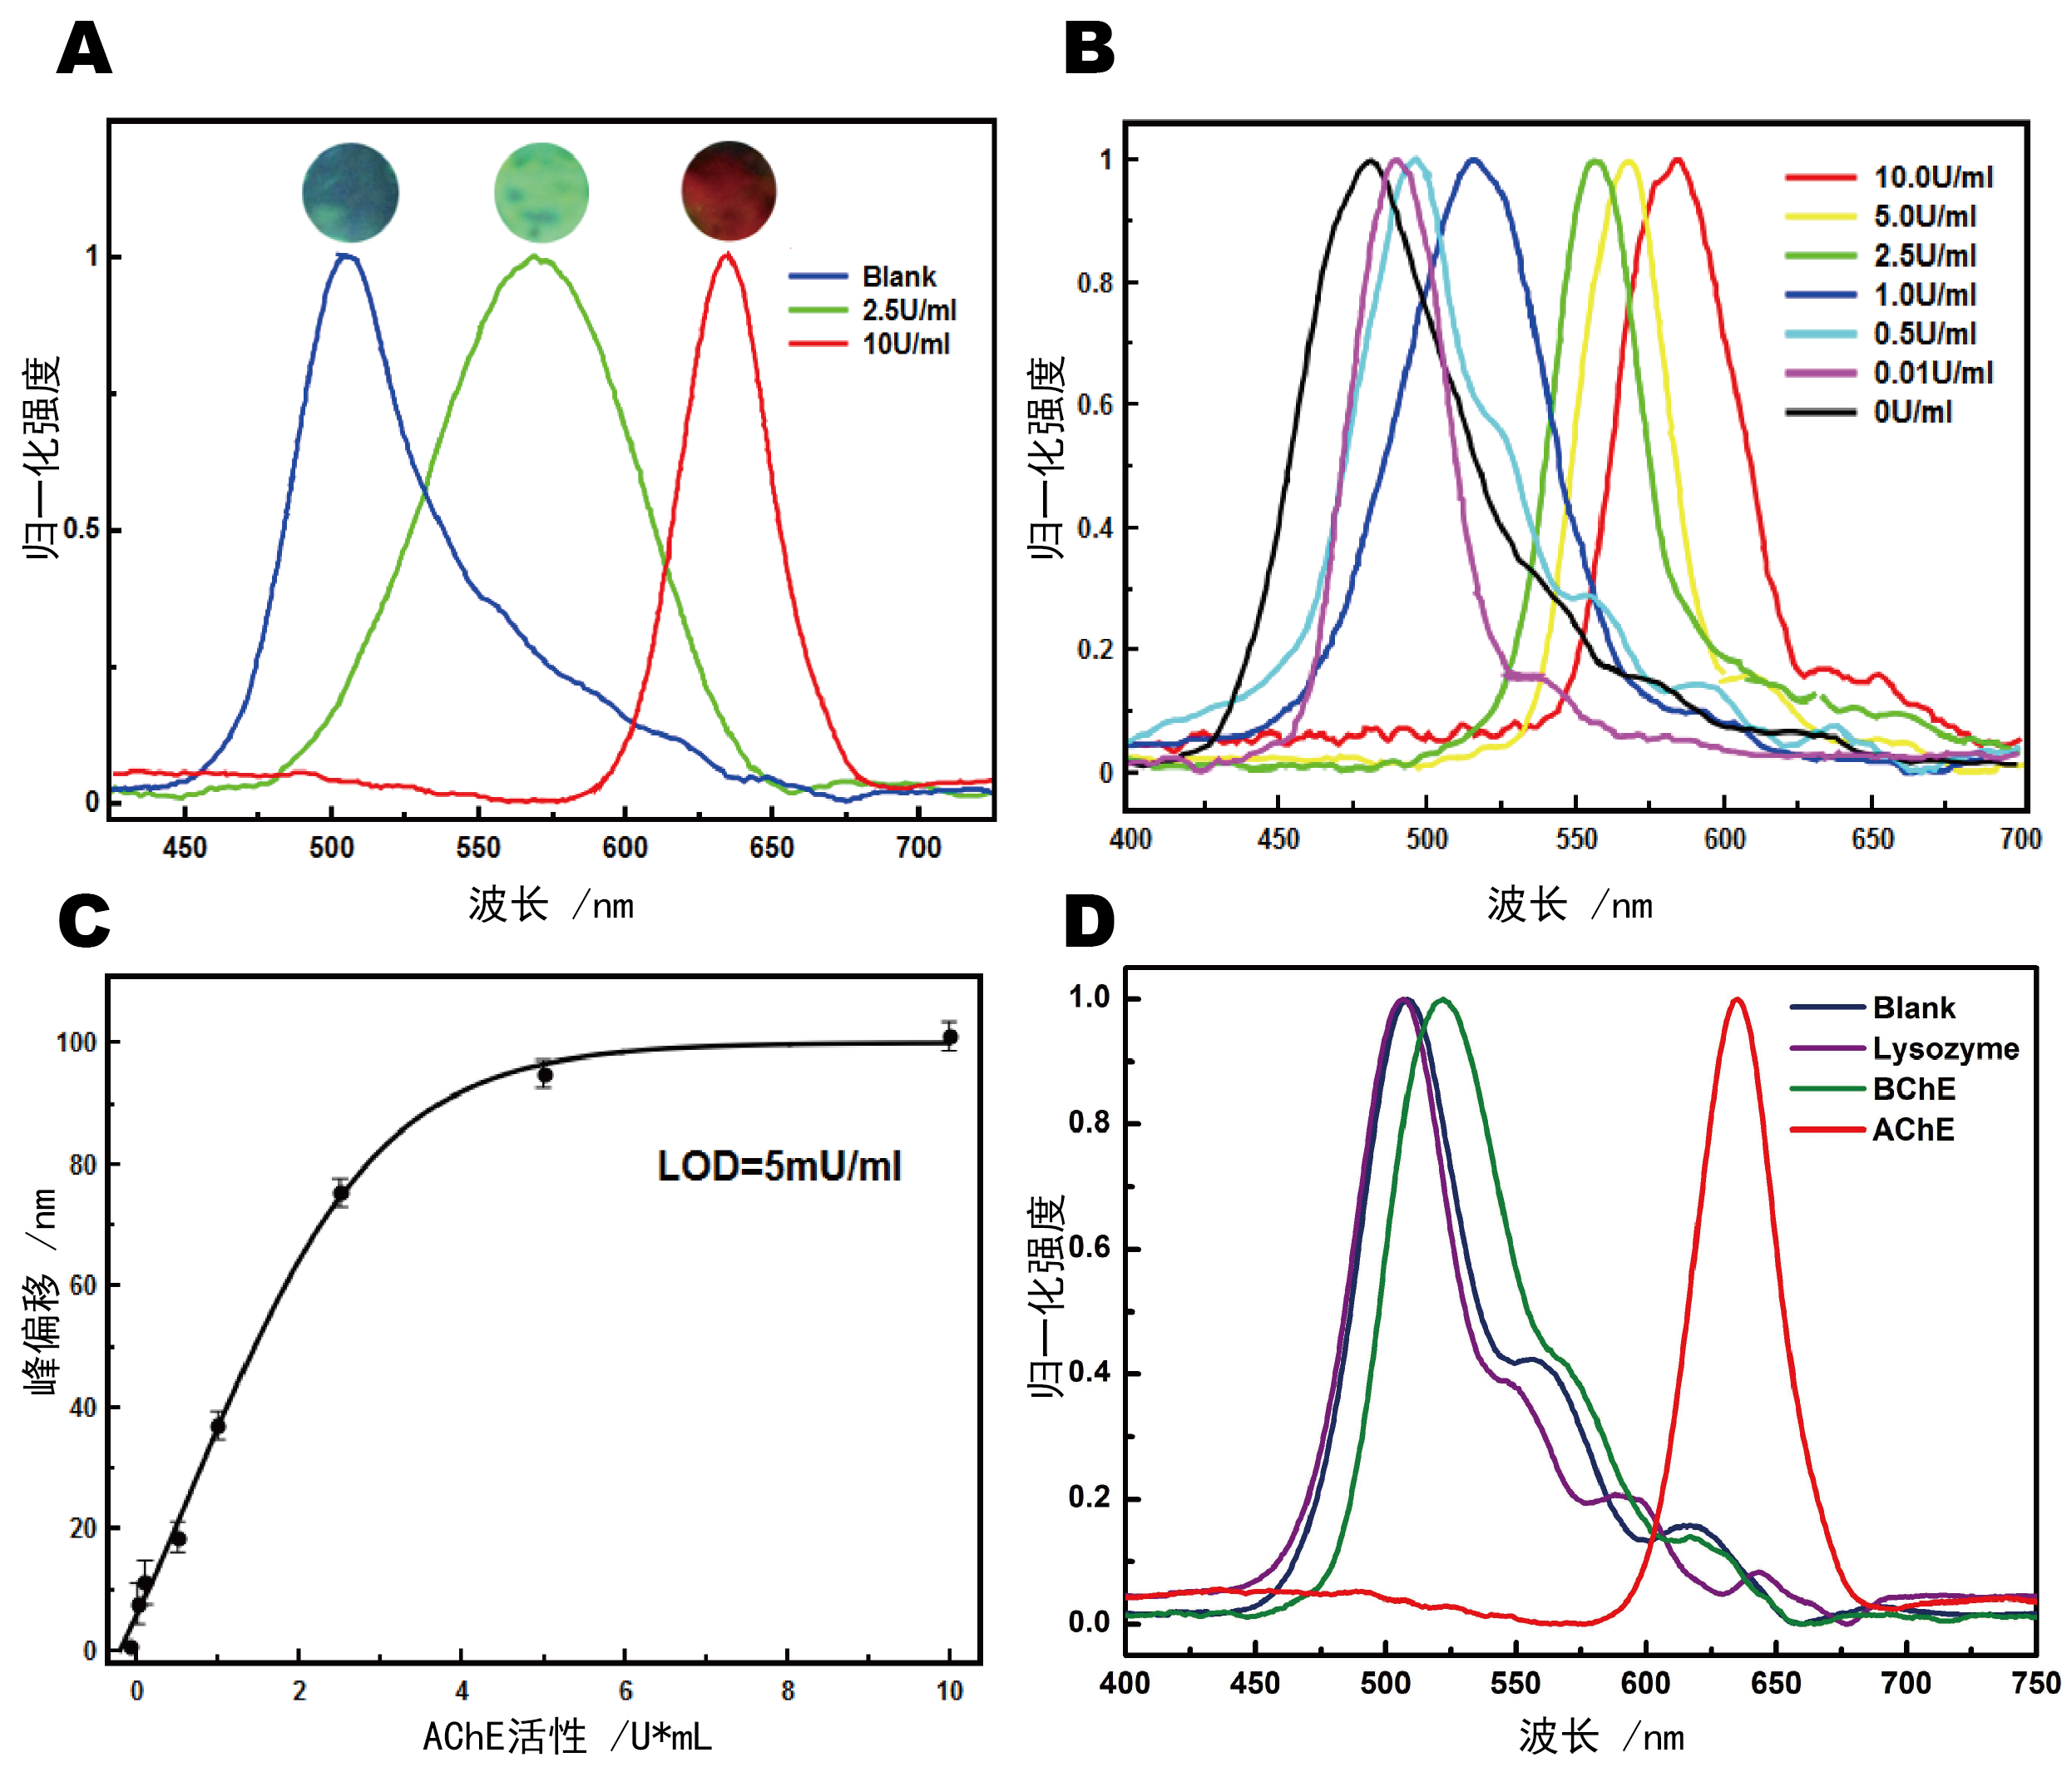
\includegraphics[width=\linewidth]{figures/ch3/enzyme_sensitivity.png}
  \caption{含马来酰亚胺的光子晶体对AChE的响应性。A. 特定AChE浓度下的Bragg衍射峰及其对应的光学照片;B. 光子晶体对不同浓度的AChE的响应性;C. B图中Bragg衍射峰-浓度对应曲线及检测极限;D 光子晶体对不同酶的选择性。}
  \label{fig:maleimide-enzyme}
\end{figure}
这种灵敏性来自于多方面的结合。首先,马来酰亚胺-巯基的反应的快速与高效特性使得光子晶体能够对含巯基的AChE水解产物产生灵敏的响应;同时,由于化学反应将含电荷的基团固定在聚合物上,使得这种修饰后的聚合物光子晶体不会受到外界溶液环境的影响;内部孔道的存在也进一步促进了活性聚合物与目标化合物的反应速率;
此外,低浓度条件下的巯基化合物也能够引起原始疏水聚合物的亲疏水性的巨大改变,这种变化保证了光子晶体检测平台的灵敏性。

最后,我们对光子晶体的检测特异性进行了表征(图~\ref{fig:maleimide-enzyme}D)。我们将光子晶体平台对溶菌酶(Lyz)、丁酰胆碱酯酶(BChE)与AChE等不同的酶的响应进行了比较。
可以发现,由于溶菌酶无法对ATCh水解,其Bragg衍射峰与空白对照组没有差别。
BChE的曲线存在一定的Bragg峰偏移,但远小于AChE的偏移量。
尽管BChE对ATCh有部分的水解,但由于速率较低,在同等时间内与AChE的结果呈现出巨大的差别。
综合上述实验结果可以说明这种含马来酰亚胺的反蛋白石光子晶体材料对于AChE具有选择性。同时,由于TCh自身的电荷与pH无关,而其他生物体内存在巯基化合物(半胱氨酸、含巯基的多肽)的电荷则随着pH存在变化,因此可以利用这种不同的pH响应性对ATCh与其余生物巯基化合物进行区分\cite{Yang2013MaleimideContaining},进一步降低了结果的假阳性水平。

\subsection{光子晶体平台对AChE酶动力学特性的检测}
上述对光子晶体性能的表征及测试展示了这种基于化学反应的光子晶体平台对AChE的检测水平。
下面将这种光子晶体平台用于一些检测应用中。
首先,我们利用光子晶体平台进行AChE的酶动力学特性的检测。
这里的目标是测定AChE的反应速率及其Michaelis-Menten速率常数。
其中,Michaelis-Menten速率方程可以表达为如下的形式:
\begin{equation}
	\label{eqn:ch3-mm}
	v=k_{cat}[E]_0\frac{[S]}{K_M+[S]}=V_{max}\frac{[S]}{K_M+[S]}
\end{equation}
其中,$V_{max}$为酶反应的最大速率,$K_M$为Michaelis-Menten常数(米氏常数),$[S]$为底物的浓度。可将公式\ref{eqn:ch3-mm}转化为如下形式:
\begin{equation}
	\label{eqn:ch3-LB}
	\frac{1}{v}=\frac{K_M+[S]}{V_{max}[S]}=\frac{K_M}{V_{max}}\frac{1}{[S]}+\frac{1}{V_{max}}
\end{equation}
本章中采用Lineweaver-Burk双倒数法法来测定$V_{max}$及$K_M$值。
可以通过对$1/[S]$-$1/v$进行线性拟合,进而从直线的斜率及截距中获得$V_{max}$与$K_M$的值。

\begin{figure}[htbp]
  \centering
  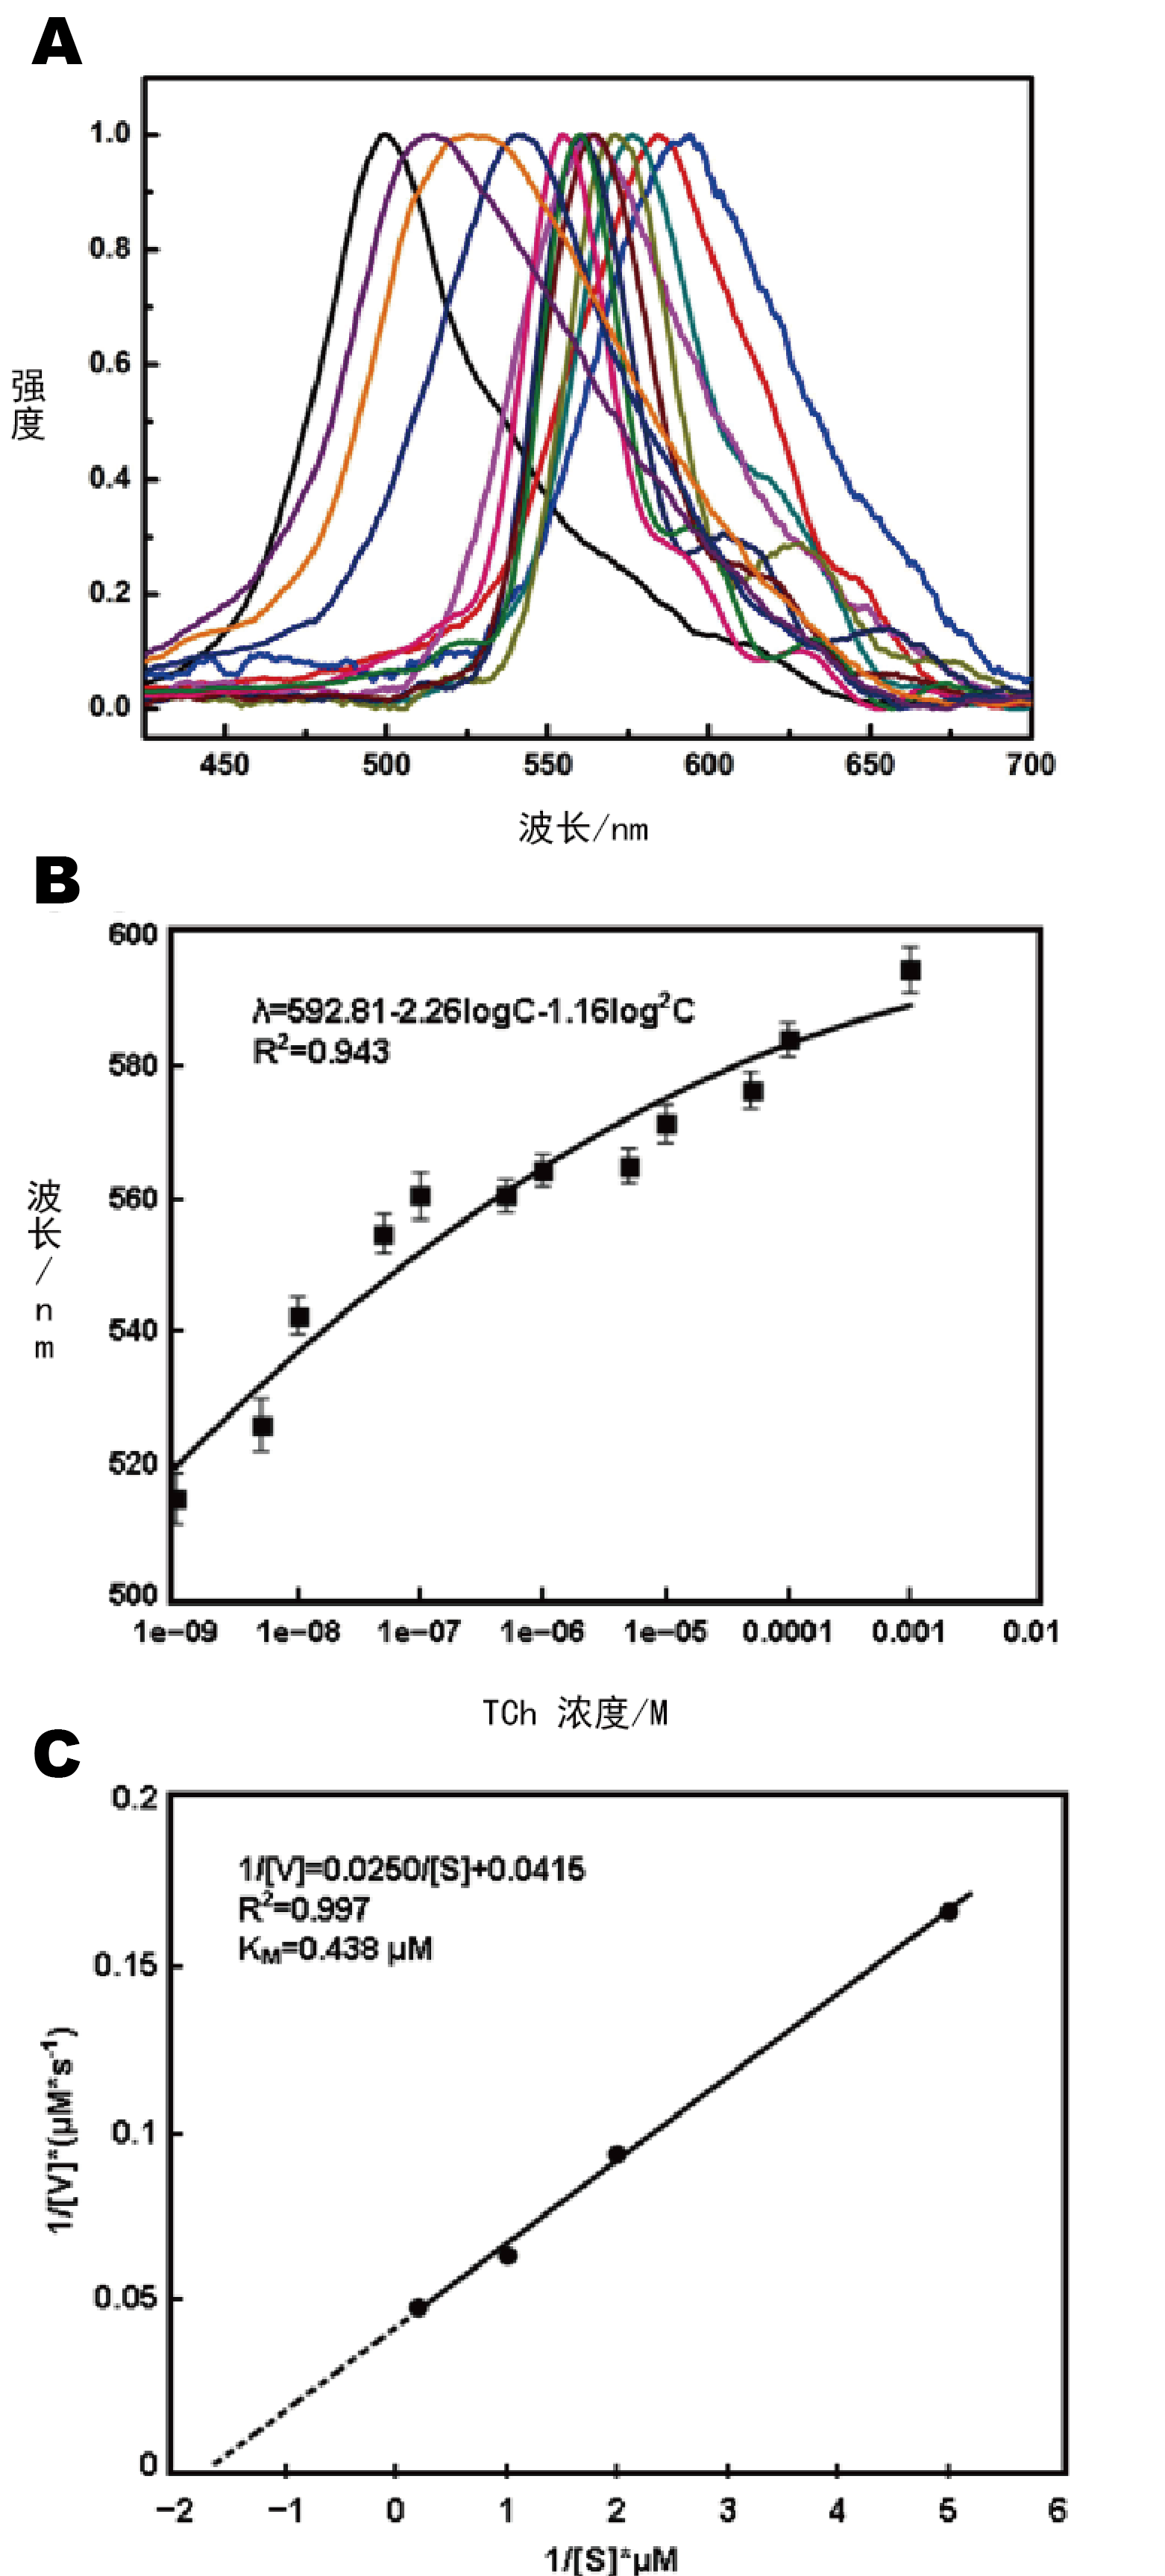
\includegraphics[height=0.8\textheight]{figures/ch3/maleimide-kinetics.png}
  \caption{含马来酰亚胺光子晶体对AChE酶动力学参数的测定。A. 不同ATCh底物浓度下的光子晶体Bragg衍射峰曲线;B. 拟合后的光子晶体标准工作曲线;C. Lineweaver-Burk双倒数法绘制的AChE动力学曲线及其参数值。}
  \label{fig:maleimide-kinetics}
\end{figure}

由于在反应速率的测定中需要对底物浓度变化进行测定,这里我们采用标准工作曲线法来获得ATCh浓度与Bragg衍射峰之间的关系,测定在不同ATCh浓度下的光子晶体响应信号。由于这里采用的AChE浓度较高(1 U/mL),在测量时间跨度内ATCh的水解已经充分,因此可以人为原始ATCh浓度等于水解的ATCh浓度。所测定的工作曲线如图~\ref{fig:maleimide-kinetics}B所示。
尽管曲线呈现出一定的Sigmoid曲线行为,对其拟合结果表明利用二次曲线拟合能够得到更高的拟合效果,并同样符合其Bragg衍射峰偏移随浓度增加而减缓的趋势。
利用测定的标准工作曲线,我们进一步测定了AChE的酶动力参数,利用不同底物浓度下的初始反应速率(以前5个数据点计算斜率)来进行双倒数拟合。
经过计算得到AChE的$V_{max}$值为40.0 µM/s,而其$K_M$值为0.438 µM(图~\ref{fig:maleimide-kinetics}C)。
所测定的米氏常数低于其他小分子标记物方法测定结果\cite{Feng2007Continuous,Wang2009Continuous}。
考虑到本实验方法的可靠性,这种差异可能来自于利用光子晶体平台时对酶的抑制水平更低。
在小分子探针化合物的情况下,小分子可能与酶的活性位点之间存在结合而产生一定的抑制;在本方法中由于光子晶体平台是一种多孔的高分子材料,不会对酶产生抑制效果,从而能够获得更低的$K_M$值(表明更高的酶活性)。

\subsection{光子晶体平台对AChE抑制剂的筛选应用}
除了对酶活性的检测以外,利用这种基于反应的光子晶体平台也能够实现对AChE抑制程度的检测,其实际意义为对不同的AChE抑制剂进行筛选,从而对阿尔兹海默症药物提供筛选依据。
对AChE的抑制水平可以通过比较同样反应时间下的正常AChE与抑制的AChE所水解的底物浓度来实现。由于水解产物能够反映为光子晶体的Bragg衍射峰位移变化,这里能够利用其光谱信号的差别来表征AChE抑制剂的抑制水平。
其中需要测定的抑制剂性能常数为其抑制效率(IE)及50\%抑制浓度(IC\text{$_{50}$})。IE表示为抑制剂结合后的酶所水解的底物浓度占正常情况下的比例:
\begin{equation}
	\label{eqn:ch3-IE}
	IE=\frac{c_0-c_i}{c_0-c_{n}}=\frac{c_{hydro,i}}{c_{hydro,n}}\approx\frac{c_{hydro,i}}{c_0}
\end{equation}
其中,下标$i$与$n$分别代表抑制与正常情况。在所选的时间跨度(30 min)内正常情况下水解的底物浓度可以近似认为等于原始浓度。
IC\text{$_{50}$}则表示为IE=50 \%时的抑制剂浓度。

\begin{figure}[htbp]
  \centering
  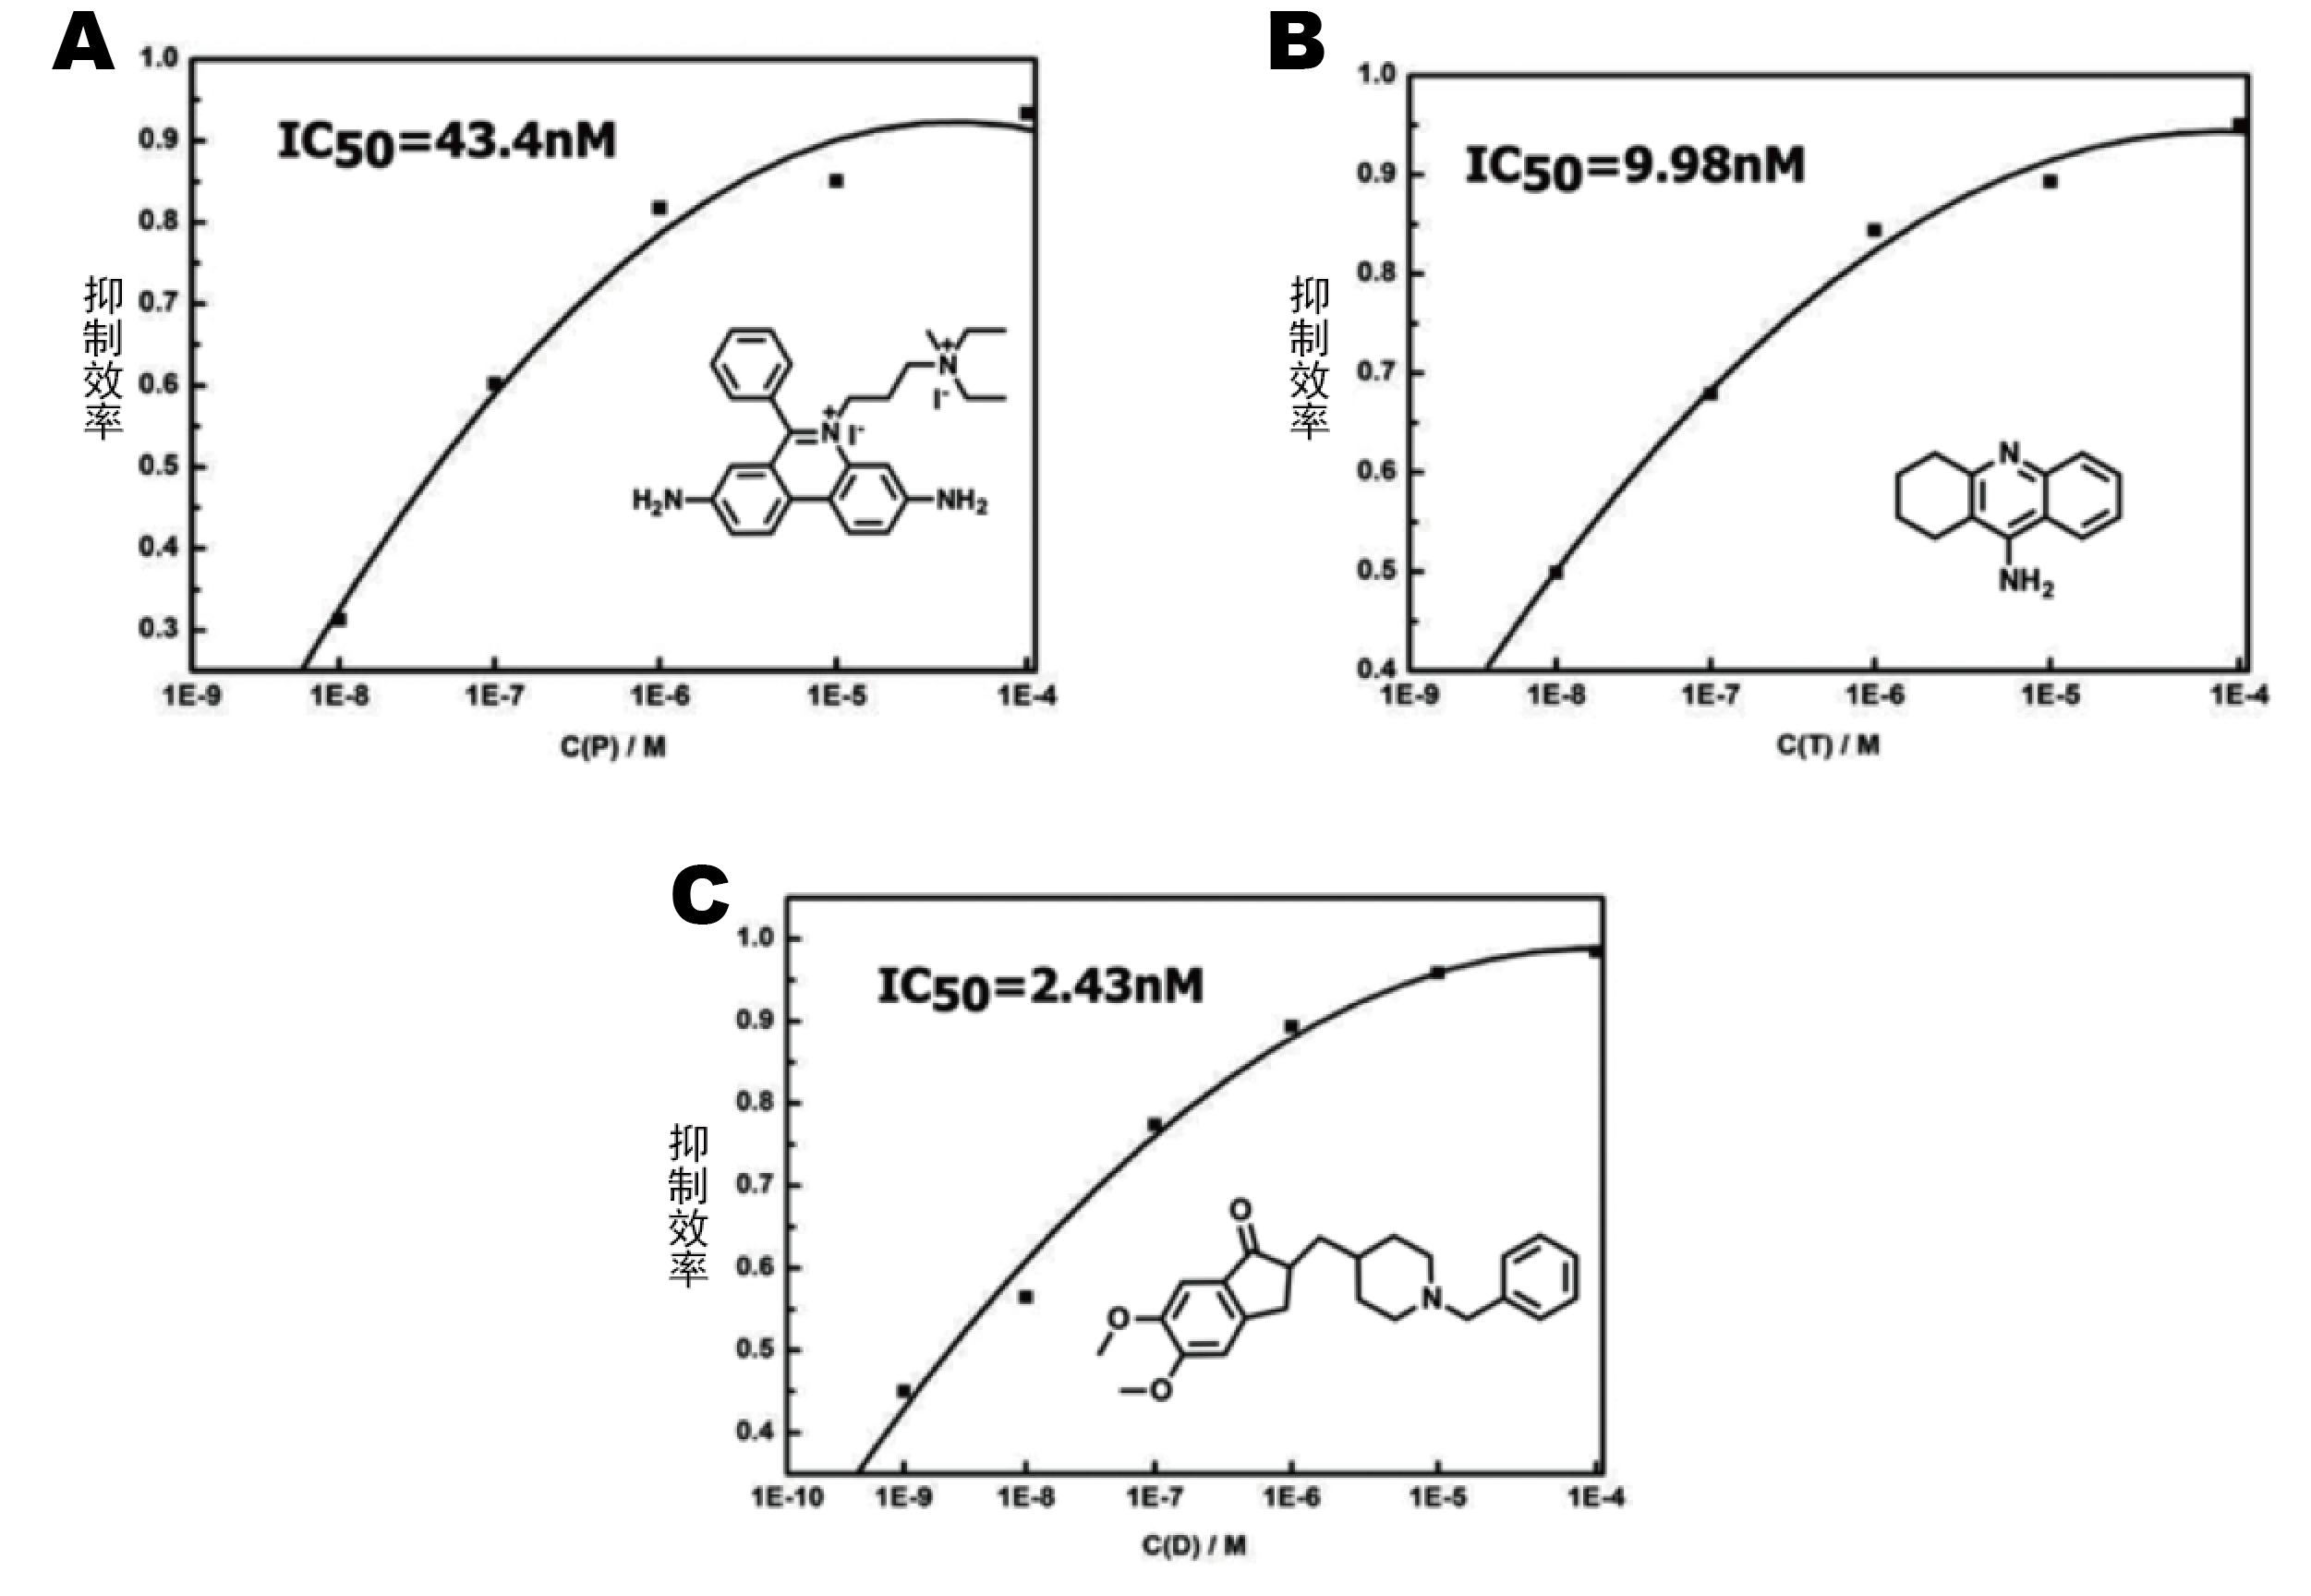
\includegraphics[width=\linewidth]{figures/ch3/inhibitor.png}
  \caption{含马来酰亚胺光子晶体对AChE抑制剂效率的测定。A. 溴化丙锭;B. 塔克林;C. 多萘哌齐。}
  \label{fig:maleimide-inhibitor}
\end{figure}

本章中,分别对三种常见的AChE抑制剂的抑制性能进行了测定,包括溴化丙锭、塔克林以及多萘哌齐。三种抑制剂的IE曲线分别如图~\ref{fig:maleimide-inhibitor}所示。根据其IE曲线可以分别将其IC\text{$_{50}$}值算出,分别为:溴化丙锭 43.4 nM,塔克林 9.98 nM,多萘哌齐 2.43nM。
可以看出多萘哌齐的抑制性能最优,塔克林次之,而溴化丙锭的抑制性能则远低于两者,体现了对抑制剂的筛选。同时,这些抑制剂的IC\text{$_{50}$}数值与其他方法测定的结果相近,证实了利用光子晶体对AChE抑制剂进行筛选的可行性。
这种方法不仅可以对阿尔滋海默症药物进行筛选,同时也可以对有毒的AChE不可逆抑制剂进行检测。与光子晶体自身的灵敏性、易操作性与信号自表达特性结合,在药物研究、临床诊断等方面具有潜在的应用。

\section{本章小结}

本章中基于马来酰亚胺-巯基反应制备了反蛋白石光子晶体材料,并用于乙酰胆碱酯酶活性检测。
结合光子晶体的光学自表达特性、化学反应对光子晶体材料的亲疏水性变化的灵敏调节,这种光子晶体检测方法具有很高的灵敏性,对乙酰胆碱酯酶活性的检测灵敏度达到5 mU/mL,在现有方法中处于前列。同时,这种光子晶体检测平台具有检测材料不依赖于液相,操作简便,信号自表达等诸多优点。此外,这种基于化学反应的光子晶体检测平台还能够适用于活性检测、酶动力学测量、抑制剂筛选等多场合应用,证明了化学反应与光子晶体结合带来的优异性能及功能材料拓展性。